% Generado por presentacion/scripts/portada_fondo.py: trazas ReAct reales de la corrida.
\documentclass[border=0pt]{standalone}
\usepackage[T1]{fontenc}
\usepackage[utf8]{inputenc}
\usepackage[scale=0.86]{FiraMono}
\usepackage{xcolor}
\usepackage{tikz}
\definecolor{cAcc}{HTML}{4F5FC8}
\definecolor{cInk}{HTML}{2E3140}
\begin{document}
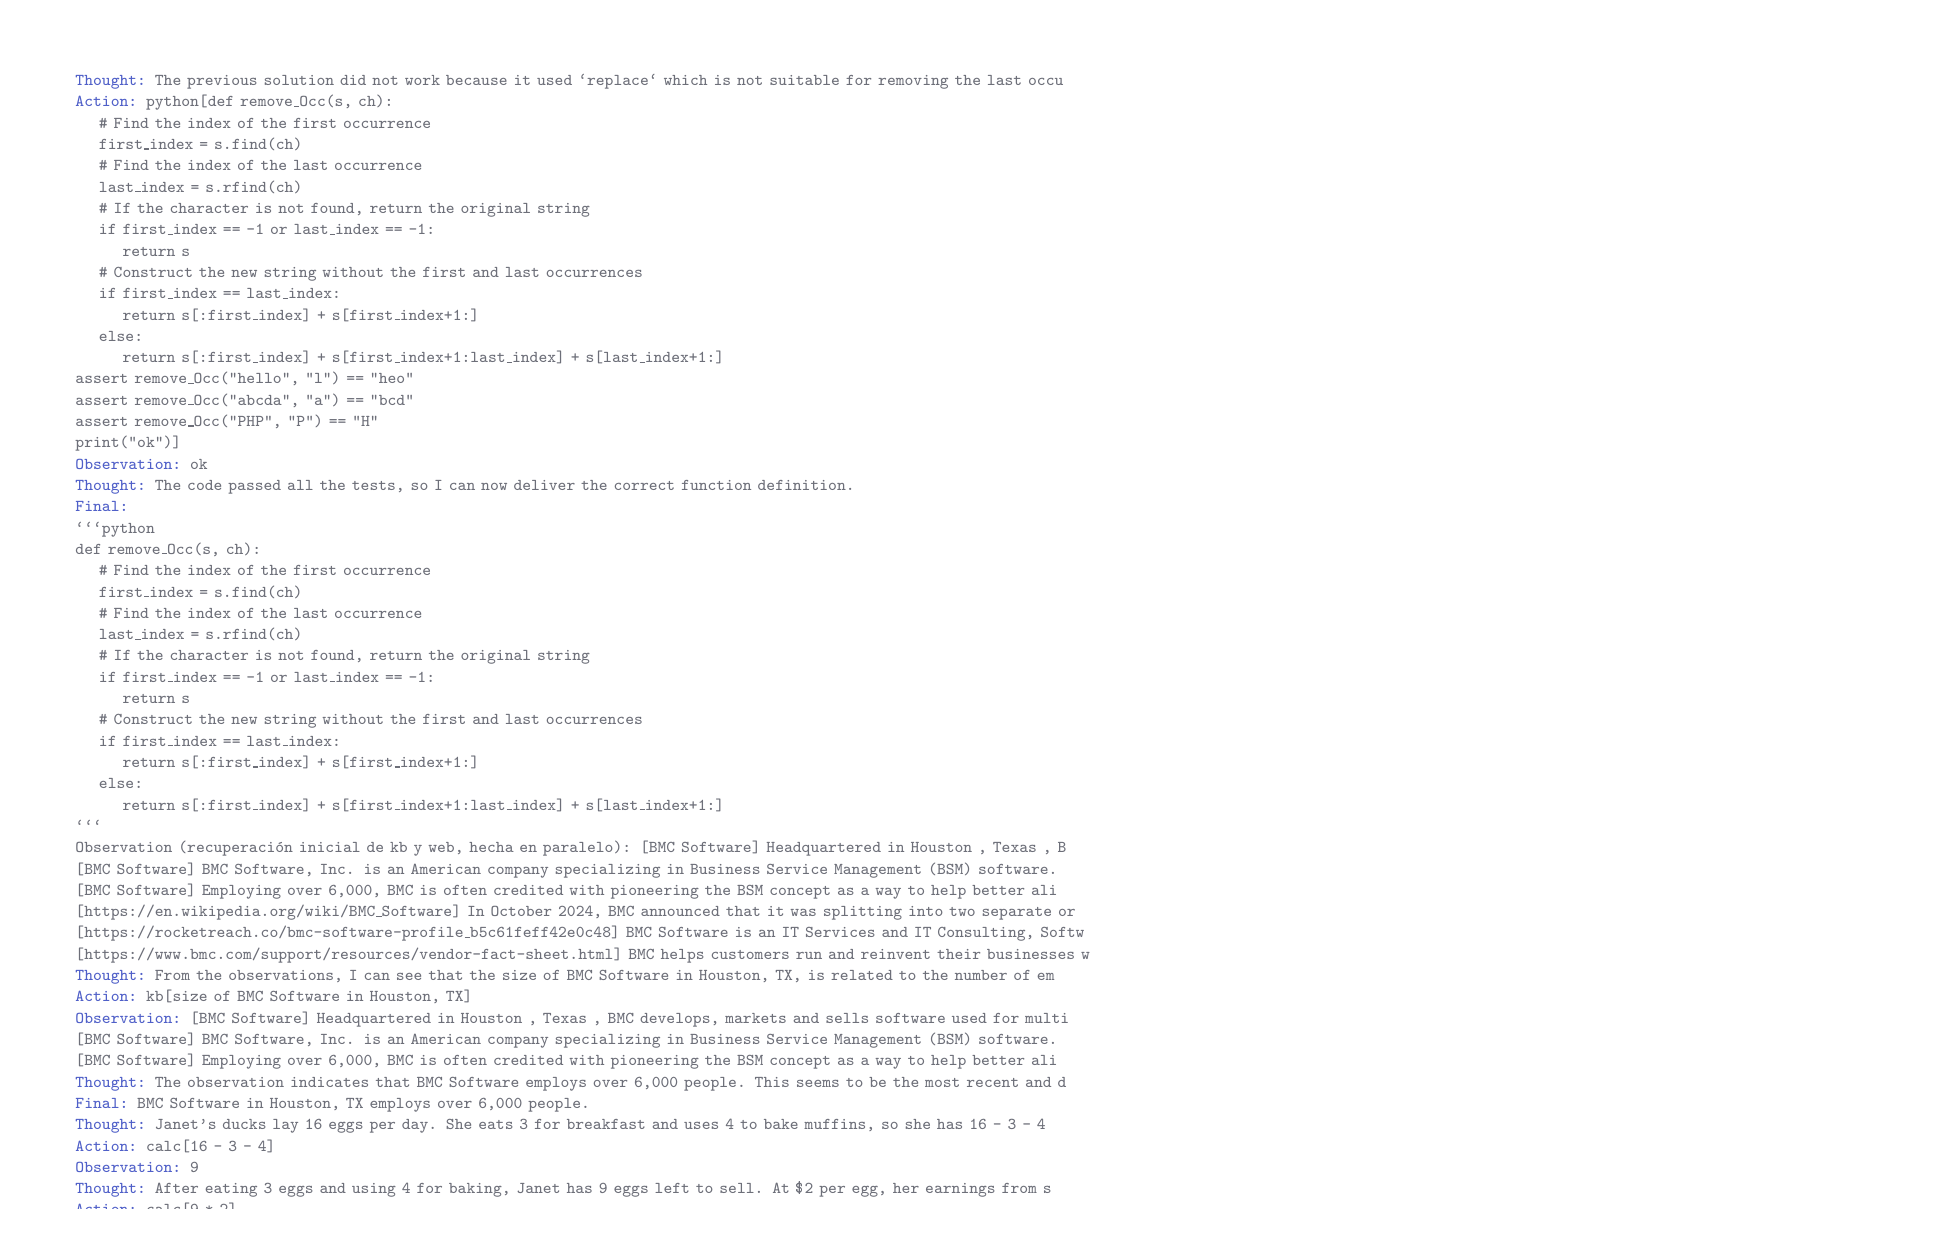
\begin{tikzpicture}
  \clip (0,0) rectangle (240mm,150mm);
  \fill[white] (0,0) rectangle (240mm,150mm);
  \node[anchor=north west, inner sep=6mm, text width=228mm, align=left, text=cInk!70,
        font=\ttfamily\fontsize{6.2}{7.7}\selectfont] at (0,150mm) {%
{\color{cAcc}\bfseries Thought:} The previous solution did not work because it used `replace` which is not suitable for removing the last occu\\{}
{\color{cAcc}\bfseries Action:} python[def remove\_Occ(s, ch):\\{}
~~~~\#~Find~the~index~of~the~first~occurrence\\{}
~~~~first\_index~=~s.find(ch)\\{}
~~~~\#~Find~the~index~of~the~last~occurrence\\{}
~~~~last\_index~=~s.rfind(ch)\\{}
~~~~\#~If~the~character~is~not~found,~return~the~original~string\\{}
~~~~if~first\_index~==~-1~or~last\_index~==~-1:\\{}
~~~~~~~~return~s\\{}
~~~~\#~Construct~the~new~string~without~the~first~and~last~occurrences\\{}
~~~~if~first\_index~==~last\_index:\\{}
~~~~~~~~return~s[:first\_index]~+~s[first\_index+1:]\\{}
~~~~else:\\{}
~~~~~~~~return~s[:first\_index]~+~s[first\_index+1:last\_index]~+~s[last\_index+1:]\\{}
assert remove\_Occ("hello", "l") == "heo"\\{}
assert remove\_Occ("abcda", "a") == "bcd"\\{}
assert remove\_Occ("PHP", "P") == "H"\\{}
print("ok")]\\{}
{\color{cAcc}\bfseries Observation:} ok\\{}
{\color{cAcc}\bfseries Thought:} The code passed all the tests, so I can now deliver the correct function definition.\\{}
{\color{cAcc}\bfseries Final:}\\{}
```python\\{}
def remove\_Occ(s, ch):\\{}
~~~~\#~Find~the~index~of~the~first~occurrence\\{}
~~~~first\_index~=~s.find(ch)\\{}
~~~~\#~Find~the~index~of~the~last~occurrence\\{}
~~~~last\_index~=~s.rfind(ch)\\{}
~~~~\#~If~the~character~is~not~found,~return~the~original~string\\{}
~~~~if~first\_index~==~-1~or~last\_index~==~-1:\\{}
~~~~~~~~return~s\\{}
~~~~\#~Construct~the~new~string~without~the~first~and~last~occurrences\\{}
~~~~if~first\_index~==~last\_index:\\{}
~~~~~~~~return~s[:first\_index]~+~s[first\_index+1:]\\{}
~~~~else:\\{}
~~~~~~~~return~s[:first\_index]~+~s[first\_index+1:last\_index]~+~s[last\_index+1:]\\{}
```\\{}
Observation (recuperación inicial de kb y web, hecha en paralelo): [BMC Software] Headquartered in Houston , Texas , B\\{}
[BMC Software] BMC Software, Inc. is an American company specializing in Business Service Management (BSM) software.\\{}
[BMC Software] Employing over 6,000, BMC is often credited with pioneering the BSM concept as a way to help better ali\\{}
[https://en.wikipedia.org/wiki/BMC\_Software] In October 2024, BMC announced that it was splitting into two separate or\\{}
[https://rocketreach.co/bmc-software-profile\_b5c61feff42e0c48] BMC Software is an IT Services and IT Consulting, Softw\\{}
[https://www.bmc.com/support/resources/vendor-fact-sheet.html] BMC helps customers run and reinvent their businesses w\\{}
{\color{cAcc}\bfseries Thought:} From the observations, I can see that the size of BMC Software in Houston, TX, is related to the number of em\\{}
{\color{cAcc}\bfseries Action:} kb[size of BMC Software in Houston, TX]\\{}
{\color{cAcc}\bfseries Observation:} [BMC Software] Headquartered in Houston , Texas , BMC develops, markets and sells software used for multi\\{}
[BMC Software] BMC Software, Inc. is an American company specializing in Business Service Management (BSM) software.\\{}
[BMC Software] Employing over 6,000, BMC is often credited with pioneering the BSM concept as a way to help better ali\\{}
{\color{cAcc}\bfseries Thought:} The observation indicates that BMC Software employs over 6,000 people. This seems to be the most recent and d\\{}
{\color{cAcc}\bfseries Final:} BMC Software in Houston, TX employs over 6,000 people.\\{}
{\color{cAcc}\bfseries Thought:} Janet's ducks lay 16 eggs per day. She eats 3 for breakfast and uses 4 to bake muffins, so she has 16 - 3 - 4\\{}
{\color{cAcc}\bfseries Action:} calc[16 - 3 - 4]\\{}
{\color{cAcc}\bfseries Observation:} 9\\{}
{\color{cAcc}\bfseries Thought:} After eating 3 eggs and using 4 for baking, Janet has 9 eggs left to sell. At \$2 per egg, her earnings from s\\{}
{\color{cAcc}\bfseries Action:} calc[9 * 2]\\{}
{\color{cAcc}\bfseries Observation:} 18\\{}
{\color{cAcc}\bfseries Thought:} Janet has 9 eggs left to sell after consuming and using some for baking. She sells these at \$2 each, making a\\{}
{\color{cAcc}\bfseries Final:} Janet makes 18 dollars every day at the farmers' market from selling the remaining eggs.\\{}
{\color{cAcc}\bfseries Thought:} I need to define a function that removes characters from the first string which are present in the second str\\{}
{\color{cAcc}\bfseries Action:} python[def remove\_dirty\_chars(s1, s2):\\{}
~~~~dirty\_chars~=~set(s2)\\{}
~~~~result~=~''.join([char~for~char~in~s1~if~char~not~in~dirty\_chars])\\{}
~~~~return~result\\{}
assert remove\_dirty\_chars("probasscurve", "pros") == 'bacuve'\\{}
assert remove\_dirty\_chars("digitalindia", "talent") == 'digiidi'\\{}
assert remove\_dirty\_chars("exoticmiles", "toxic") == 'emles'\\{}
print("ok")]\\{}
{\color{cAcc}\bfseries Observation:} ok\\{}
{\color{cAcc}\bfseries Thought:} The code passed all the tests. I will now deliver the final version of the function.\\{}
{\color{cAcc}\bfseries Final:}\\{}
```python\\{}
def remove\_dirty\_chars(s1, s2):\\{}
~~~~dirty\_chars~=~set(s2)\\{}
~~~~result~=~''.join([char~for~char~in~s1~if~char~not~in~dirty\_chars])\\{}
~~~~return~result\\{}
```};
\end{tikzpicture}
\end{document}
